\documentclass[aspectratio=169,12pt]{beamer}
\usepackage[utf8]{inputenc}
\usepackage{graphicx}
\usepackage{tikz}
\usepackage{listings}
\usepackage{hyperref}
\usepackage{booktabs}
\usepackage{multicol}
\usepackage{xcolor}
\usepackage{verbatim}
\usepackage{fontawesome5}

\usetheme{Madrid}
\usecolortheme{whale}
\setbeamertemplate{navigation symbols}{}

\title{Day 1: Web Application Architecture and Fundamentals}
\subtitle{Comprehensive Training with Practical Examples and Hands-on Exercises}
\author{Security Training Team}
\institute{Web Application Security Department}
\date{\today}

\begin{document}

\begin{frame}
\titlepage
\end{frame}

\begin{frame}{Training Objectives}
\begin{columns}
\column{0.5\textwidth}
\textbf{Learning Outcomes:}
\begin{itemize}
\item[\faIcon{check-circle}] Understand web application architecture components
\item[\faIcon{check-circle}] Identify security implications of different architectures
\item[\faIcon{check-circle}] Analyze component interactions and data flow
\item[\faIcon{check-circle}] Apply security architecture principles
\end{itemize}
\column{0.5\textwidth}
\textbf{Practical Skills:}
\begin{itemize}
\item[\faIcon{laptop-code}] Architecture analysis techniques
\item[\faIcon{tools}] Security assessment methodologies
\item[\faIcon{shield-alt}] Security implementation strategies
\item[\faIcon{clipboard-check}]{Hands-on lab exercises}
\end{itemize}
\end{columns}
\end{frame}

\begin{frame}{Web Application Architecture Overview}
\begin{columns}
\column{0.6\textwidth}
\textbf{Core Architecture Components:}
\begin{enumerate}
\item \textbf{Client-Side Layer}
\begin{itemize}
\item Web browsers and mobile clients
\item Frontend frameworks and libraries
\item User interface components
\end{itemize}
\item \textbf{Server-Side Layer}
\begin{itemize}
\item Web servers (Apache, Nginx, IIS)
\item Application servers (Tomcat, WildFly)
\item API gateways and load balancers
\end{itemize}
\item \textbf{Data Layer}
\begin{itemize}
\item Databases (SQL, NoSQL)
\item Caching systems (Redis, Memcached)
\item File storage and object storage
\end{itemize}
\item \textbf{Infrastructure Layer}
\begin{itemize}
\item Network components and firewalls
\item Cloud services and containers
\item Monitoring and logging systems
\end{itemize}
\end{enumerate}
\column{0.4\textwidth}
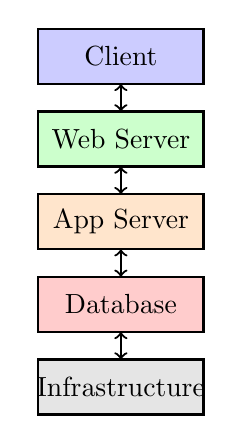
\begin{tikzpicture}[scale=0.7]
\draw[thick, fill=blue!20] (0,4) rectangle (3,5) node[pos=.5] {Client};
\draw[thick, fill=green!20] (0,2.5) rectangle (3,3.5) node[pos=.5] {Web Server};
\draw[thick, fill=orange!20] (0,1) rectangle (3,2) node[pos=.5] {App Server};
\draw[thick, fill=red!20] (0,-0.5) rectangle (3,0.5) node[pos=.5] {Database};
\draw[thick, fill=gray!20] (0,-2) rectangle (3,-1) node[pos=.5] {Infrastructure};
\draw[<->,thick] (1.5,4) -- (1.5,3.5);
\draw[<->,thick] (1.5,2.5) -- (1.5,2);
\draw[<->,thick] (1.5,1) -- (1.5,0.5);
\draw[<->,thick] (1.5,-0.5) -- (1.5,-1);
\end{tikzpicture}
\end{columns}
\end{frame}

\begin{frame}{Summary and Key Takeaways}
\begin{columns}
\column{0.5\textwidth}
\textbf{Architecture Fundamentals:}
\begin{itemize}
\item[\faIcon{building}] Understanding web app layers
\item[\faIcon{network-wired}] Component interactions
\item[\faIcon{sitemap}] Data flow mapping
\item[\faIcon{cogs}] Technology selection impact
\end{itemize}
\textbf{Security Considerations:}
\begin{itemize}
\item[\faIcon{shield-alt}] Defense in depth
\item[\faIcon{key}] Least privilege principle
\item[\faIcon{lock}] Fail secure approach
\item[\faIcon{eye}] Zero trust architecture
\end{itemize}
\column{0.5\textwidth}
\textbf{Practical Implementation:}
\begin{itemize}
\item[\faIcon{code}] Secure coding practices
\item[\faIcon{tools}]{Security tool integration}
\item[\faIcon{clipboard-check}]{Regular security assessments}
\item[\faIcon{book}]{Documentation and policies}
\end{itemize}
\textbf{Next Steps:}
\begin{itemize}
\item[\faIcon{arrow-right}] Apply concepts to real projects
\item[\faIcon{arrow-right}] Conduct security audits
\item[\faIcon{arrow-right}] Implement security controls
\item[\faIcon{arrow-right}]{Continuous improvement}
\end{itemize}
\end{columns}
\vspace{0.5cm}
\begin{center}
\Large{\textbf{Questions?}}\\
\vspace{0.3cm}
\normalsize{Contact: security-team@organization.com}\\
\vspace{0.2cm}
\small{Additional Resources: OWASP Foundation, NIST Cybersecurity Framework}
\end{center}
\end{frame}

\end{document}